dump of potentially useful writings

\begin{equation}
g^{\alpha\beta}g^{\gamma\delta}R_{\alpha\mu\gamma\nu}
    =\tensor{R}{^\beta_\mu^\delta_\nu}
\end{equation}

%\section*{Future Work}
%Including external datasets in training to see how performance on held out molecules in the external sets and if there is any performance degradation on molecules held out from the Biobyte Star Set. This model might replace the existing package implementation allowing more accurate predictions over a wider range of logP values.
%
%Taking account of the variance in measured logP values of the closest $N$ neighbours or how the model fairs (also the error on the nearest neighbour)
%
%Use multiple instances of the model types in the ensemble, not only the best ones.
%Try different meta models, maybe more complex ones, not only GLM
%Why do you think GBM and SVM are ensembled together… are they somehow of a different form.
%Recommend that other algorithms get ensembled in the same way instead of just taking an average.

\subsection*{Learning curves}
The effect of training set size on model performance was investigated by randomly selecting training data from the training set. This was done in steps of 1000 molecules. At each step the random subset was split into a training and holdout set consisting of 4/5 and 1/5 of the data respectively. Gaussian process regression was trained at each step as this requires only a single hyper-parameter to be tuned. 5 fold cross validation was performed on the training set and the model with the lowest cross-validated RMSE was used to make predictions on the holdout set. There was a clear trend of increasing model performance with increasing training set size. Compared with the performance trend using cross-validation, the test set performance exhibits more random fluctuation since it is not averaged over the 5 cross validation folds.

\subsection*{Learning curves}
The effect of training set size on model performance was investigated by randomly selecting training data from the training set (Figure \ref{fig:learning_curves}). This was done in steps of 1000 molecules. At each step the random subset was split into a training and holdout set consisting of 4/5 and 1/5 of the data respectively. Gaussian process regression was trained at each step as this requires only a single hyper-parameter to be tuned. 5 fold cross validation was performed on the training set and the model with the lowest cross-validated RMSE was used to make predictions on the holdout set. There was a clear trend of increasing model performance with increasing training set size. Compared with the performance trend using cross-validation, the test set performance exhibits more random fluctuation since it is not averaged over the 5 cross validation folds.

\begin{figure}[ht]
  \centering
  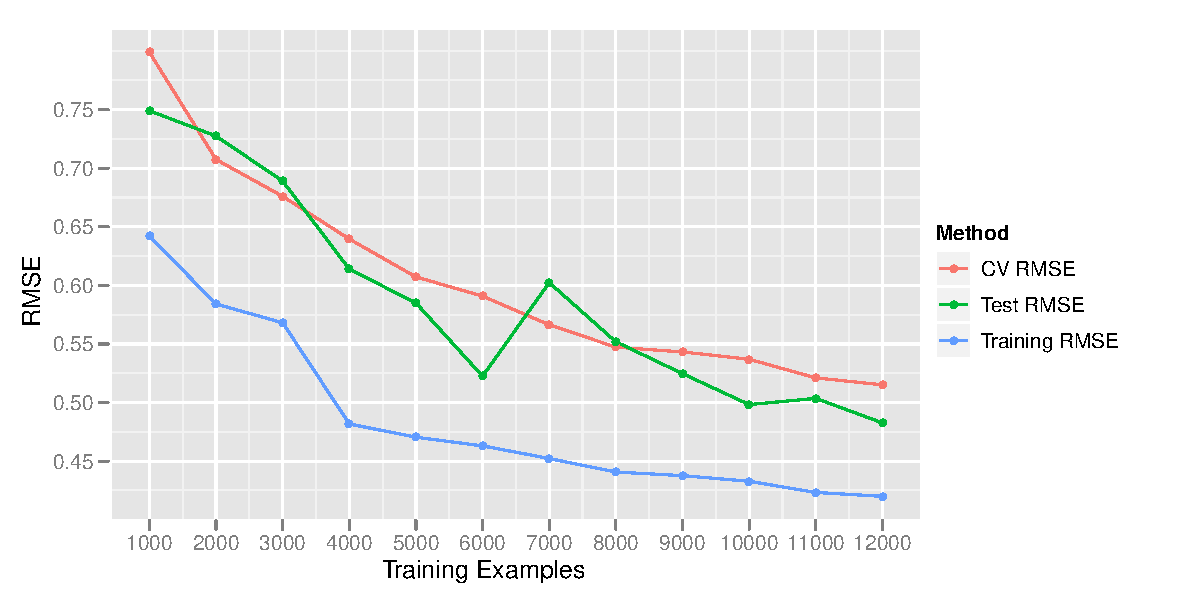
\includegraphics[width=0.7\textwidth]{./Figures/learning_curves.pdf}
  \caption{Gaussian process regression accuracy increases as the size of random subsets increase. RMSE is used as the performance metric to compare the performance between the model on the training set (4/5 of the random subset), holdout set (1/5 of the random subset) and in 5 fold cross-validation (CV) over the training set.}
  \label{fig:learning_curves}
\end{figure} 

\subsection*{Data preparation}
Out of the initial 12,570 molecules used for training, the filtering procedure removed 124 inorganic molecules. 2 with molecular weight below 20 Da, 13 with molecular weight above 900 Da. 239 with more than 3 Chlorines, 8 with more than 3 Bromines, 71 with more than 3 Fluorines and 15 duplicates leaving 12098 molecule-target pairs for training. PaDEL-Descriptor took 6 minutes and 16 seconds to calculate 729 descriptors for each of the 12098 remaining molecules when run over 14 Intel Xeon E5520 2.27GHz cores. Simple random sampling was performed, dividing the initial set into 9678 molecules for the training set and 2420 molecules for the holdout set. 

6 of the logP related descriptors were removed, 362 descriptors were removed due to low variance and 127 descriptors were removed because of their high correlation to other descriptors. The remaining 234 descriptors were used to train the models. These descriptors are listed in SI Table 1.

\subsection*{Support vector regression}

Support vector regression is an extension of support vector machines which were developed by Vapnik and Cortes \cite{cortes_support-vector_1995} to perform non-linear binary classification. SVMs employ a kernel function ($\phi$) which casts the original data into a higher dimensional space where the data is separated 'as best as possible' by a hyperplane that maximises the distance from the closest input vectors (support vectors). The most popular and well performing kernel function is the radial basis function which is usually of the form $K(x,y) = e^{-\sigma||x-y||^2}$ where sigma is a hyper-parameter that defines the width of the function.

Support Vector Regression, instead of using a hyperplane to separate the data in the higher dimensional space, uses ordinary least squares or partial least squares regression in that space to find a linear relationship between the new feature vectors and the target. The cost function that is minimised to obtain the best regression model is made up of two components: a loss function and a smooth regularisation term and the goal is to minimise both the size of the coefficients (smoothness) and the prediction errors (accuracy). Another hyper-parameter requiring adjustment is the error weight $C$ which controls the importance of smoothness vs accuracy. If C is high, accuracy is favoured and smoothness is neglected resulting in a model that will over-fit the training data. To make sure that over-fitting is not occurring, SVR relies upon re-sampling techniques to find the optimal hyper-parameters $\sigma$ and $C$. 

Vapnik uses an $\epsilon$-insensitive loss functiosn where only data points with predictions which deviate more than $\epsilon$ are taken into account. In the SVR context, only these data points are called support vectors and only these data points determine the final training of the SVR model.

Advantages of SVMs and SVR are that, once trained, they are fast at predicting new data points since they only rely on their support vectors. For a more detailed theoretical background on SVMs and SVR, the reader is referred to \cite{cristianini_introduction_2000}. 

\subsection*{Generalized boosted regression}

Write up a section about how generalized boosted regression works.

(Rough language, will be cleaned) Figure \ref{fig:error_estimation} shows the relationship between $D$, the average distance of the molecule in a test set to the closest $x$ molecules in the training set, and $\sigma$, the estimated width of the gaussian at that distance (using the windowed process as explained in the methods section). $\sigma$ estimates using molecules from the external test set seem to map to two regions in the distance space, that is: $D < 16$ and $D > 16$. A line was fit to each of these regions using simple linear regression. For a new molecule, $D$ can be calculated and the fit in the corresponding region can be used to estimate a $\sigma$ for the gaussian that will provide the distribution of error for that molecule around its predicted value. QUESTION: could the change in slope be an artefact of the method used here or do you think it's naturally inherent in the data.

For molecules that exceed a $D$ of 16, the accuracy in prediction falls off at a steeper rate than those molecules closer to the training set. This could be described at a domain of reduced applicability of the model and a warning given after prediction.

It is interesting to note that the fit to molecules in the holdout test set (Internal) is both lower and flatter. This could be due to a combination of factors. Firstly the molecules are drawn from the different distribution from the training set and correlations between descriptors and the target value are likely to be different when drawing molecules from this distribution compared with taking molecules from a random sample of the training data. Secondly, the distribution of the target value if much wider in the external test set (see figure \ref{fig12}) so the model is lacking data in areas when logP is extreme.

For purposes of model use, the fits to the external test set will be used to estimate $\sigma$'s for new molecules. It cannot be guaranteed that the correlation between the descriptors and the target value of molecules drawn from a distribution that is different to that of the external test set is the same as the relationship between the training set and the external test set, but this could be considered the best estimate with the data available (TBD: very bad wording need to fix).

%(TBD: mention previous approaches to the applicability domain problem.)
%To obtain an estimate of the prediction error for new molecules a nearest neighbour approach was adopted. The errors used in this approach are the difference between the predictions using SVR and logP values from the external test set obtained from the PKKB. The approach assumes a Gaussian distribution for the error and tries to find a relationship between the standard deviation, $\sigma$, and the average Euclidean distance to a subset (size ranging from 1 to 5) of closest molecules in the training set, $D$. The average Euclidean distance is found by averaging the Euclidean distance found using the normalised form of all the descriptors used in model training. For each molecule in the external test set, windows were constructed which include all molecules whose D only differs by the at most half the window width. For each molecule, 10 windows were used ranging from width 1 to 2 distance units in fixed intervals. If there were more than 10 molecules inside a window then a Gaussian was fitted to the prediction errors of these molecule using maximum likelihood estimation, fixing the mean of the Gaussian to zero. This was achieved by finding a maximum of the function:
%
%\begin{equation}
%	\label{eq:liklihood}
%	L(\theta|error_1,…,error_n) = \prod_{i=1}^{n}{f(error_i|\theta)} = \prod_{i=1}^{n}{\frac{1}{{\sigma \sqrt {2\pi } }}e^{{{ - \left( {error_i - 0 } \right)^2 } \mathord{\left/ {\vphantom {{ - \left( {x - \mu } \right)^2 } {2\sigma ^2 }}} \right. \kern-\nulldelimiterspace} {2\sigma ^2 }}}}
%\end{equation}
%
%Each estimated $\sigma$ per window contributed towards an average $\sigma$ for that molecule. In this way, a $\sigma$ vs $D$ relationship was achieved. Linear regression was used to fit this relationship to obtain a model which predicts $\sigma$ given the average Euclidean distance to a subset of closest molecules in the training set. 

, with cross-validated root-mean-squared-errors of 0.4 log units and 0.45 log units respectively.

% \subsection*{Comparison to other methods} taken out to make this one section	
% (Rough language, will be cleaned) The SVR model compares favourably with existing methods of logP prediction. Table \ref{tab:external_comparison} shows the performance of existing methods on the external test set. SVR is measurably superior to logP predictions given by the MOE and PaDEL-Descriptor package. Is is interesting to note the stark difference in the performance of the AlogP implementations from pipeline pilot and PaDEL-Descriptor. This shows that similar named prediction tools cannot be trusted to produce the same results.  AlogPS performs the best out of all the method but it is uncertain how many of the external test set molecules were used in the training of this model. A (TBD: think about another name for chear) cheat version of the SVR model is included which add all the external test set molecules to the training set. For comparison, this provides a lower bound on the performance of algorithms that already include all of the external test set molecules in their training.

%\begin{itemize}
%\item AlogP, MlogP and XlogP as calculated by the PaDEL-Descriptor program.
%\item logP.o.w and SlogP as calculated by the Molecular Operating Environment.
%\item AlogP as calculated by Pipeline Pilot.
%\item AlogPS calculated through Tetko’s online service (ref).
%\end{itemize}

\begin{itemize}
\item Molecules were read in either SMILES or SDF format.
\item Hydrogens were made implicit through the use of the \textit{indigoFoldHydrogens} method. 
\item Molecules were excluded if they did not pass the Indigo checks for correct valence or ambiguous Hydrogens as determined by the methods \textit{indigoCheckBadValence} and \textit{indigoCheckAmbiguousH} respectively.
\item Atomic isotopes were converted to their common forms using the \textit{resetIsotopes} method. 
\item Molecules were excluded if they contained any atoms not in \{H, C, N, O, P, S, F, Cl, Br, I\}. 
\item Indigo's de-aromatise algorithm was invoked,  converting molecules stored using aromatic bonds to a kekulised form.
\item De-aromatised molecules were converted to their Inchi representation \cite{_iupac_????} using Indigo's Inchi plugin. 
\item All Inchi layers below and including the tautomeric layer were removed.
\item SMILES were constructed using this shortened Inchi, thus converting multiple tautomeric forms to a single form. 
\item Molecules were excluded if they had a molecular weight less than 20 Da or greater than 900 Da. 
\item Molecules were excluded if they contained more than 3 of any one halogen. In particular, the training set contained 239 molecules containing more than three Chlorine atoms, so this operation made the training set more representative of small organic molecules that were likely to be used as drugs, for example.
\item Negative charges on oxygens bonded to any of Carbon, Sulphur or Phosphorus were removed (using SMARTS pattern [O-\$(*[\#6,\#14,\#15])]), neutralising these negatively charged acidic groups.
\item Positive charges on $NH_2$ groups were removed (using SMARTS pattern [\#7+\$(*[H])]), neutralising these positively charged nitrogen bases.
\item Salts were removed by isolating connected components and removing all but the largest component.
\item Duplicates were removed if they had matching canonical SMILES. 
\item Molecules were written out in SDF format.
\end{itemize}

\section*{A Coarse Review of Computational Approaches to Predict LogP}

\subsection*{Hansch and Fujita's $\pi$-System}

\subsection*{Fragment based methods}

\subsection*{Atom-based methods}

\subsection*{Whole molecule approches}

\subsection*{Recent comparison of existing methods}

\section*{Approach Adopted Here}

% 10 MOST IMPORTANT DESCRIPTORS TABLE
\begin{table}[htbp]
  \centering
  \caption{Method performance on external test set. SVR Model Cheat incorporates the external test set molecules into the training set. Since other methods may include some of the external test set molecules in their training sets, this cheat method is included as a guide to see how well a method should do if it included all of these molecules. (TBD: these need to be recalculated on trimmed external test set, need to add more methods here.)}
    \begin{tabular}{lr}
    \toprule
    Method & RMSE \\
    \midrule
    AlogP (PaDEL-Descriptor) & 3.3 \\
    MlogP (PaDEL-Descriptor) & 2.8 \\ 
    XlogP (PaDEL-Descriptor) & 2.5 \\
    AlogP (Pipeline Pilot) & 1.8 \\
    SLogP (MOE) & 2.5 \\
    LogP (o/w) (MOE) & 2.6 \\
    AlogPS (Tetko) & 0.96 \\
    SVR Model & 1.2 \\
    SVR Model Cheat & 0.47 \\
    \bottomrule
    \end{tabular}%
  \label{tab:external_comparison}%
\end{table}% 

%Out of the 1012 molecules with measured logP values from the external dataset collected from the PKKB database, 16 molecules were removed because they have duplicate canonical SMILES within the external dataset, 31 were considered as being too large ($>$900 Da) and out of the scope of the model, 5 were removed because they contain more than 3 Chlorine atoms, 10 were removed because they contain more than 3 Fluorine atoms, 201 were removed because they were duplicates by canonical SMILES of molecules in the training set and a further 238 were removed because they were tautomers of molecules in the training set. It is important to remove these tautomeric duplicates as their inclusion results in an artificial increase in model performance on the external test set. Sending both the training set and the external test set through the same standardisation procedure which, using Indigo's IUPAC InChI plugin, converts molecules to their unique tautomeric form allows the removal of these duplicates.  
%
%On the remaining 521 external test molecules (TBD: provide these in SI as a data file), the SVR model performs with an RMSE of 1.091. Figure \ref{fig:error_analysis} shows a measured vs predicted correlation plot highlighting molecules of interest. Manually inspecting molecules with high prediction error revealed mistakes in the structural representation for Diltiazem and Verapamil in the PKKB database. Correcting these structures results in remarkably accurate predictions for these molecules (TBD: mention corrected values and their deviation from experimental measurement). Also, multiple molecules containing charged tetravalent nitrogens were found in the external test set. Since it is not possible to experimentally measure the logP of these molecules in their neutral form (TBD: double check this is actually the case), they can be considered out of the scope of the model. When molecules containing tetravalent nitrogens are removed and the two incorrect structures are corrected the RMSE of the SVR model drops to 0.871. This modified external test set is used to compare the SVR model with existing models.
%
%(TBD: Say something about the density plot and why the prediction towards the lower and higher ranges of logP are off.)

%\begin{figure}
%\centering
%\mbox{\subfigure{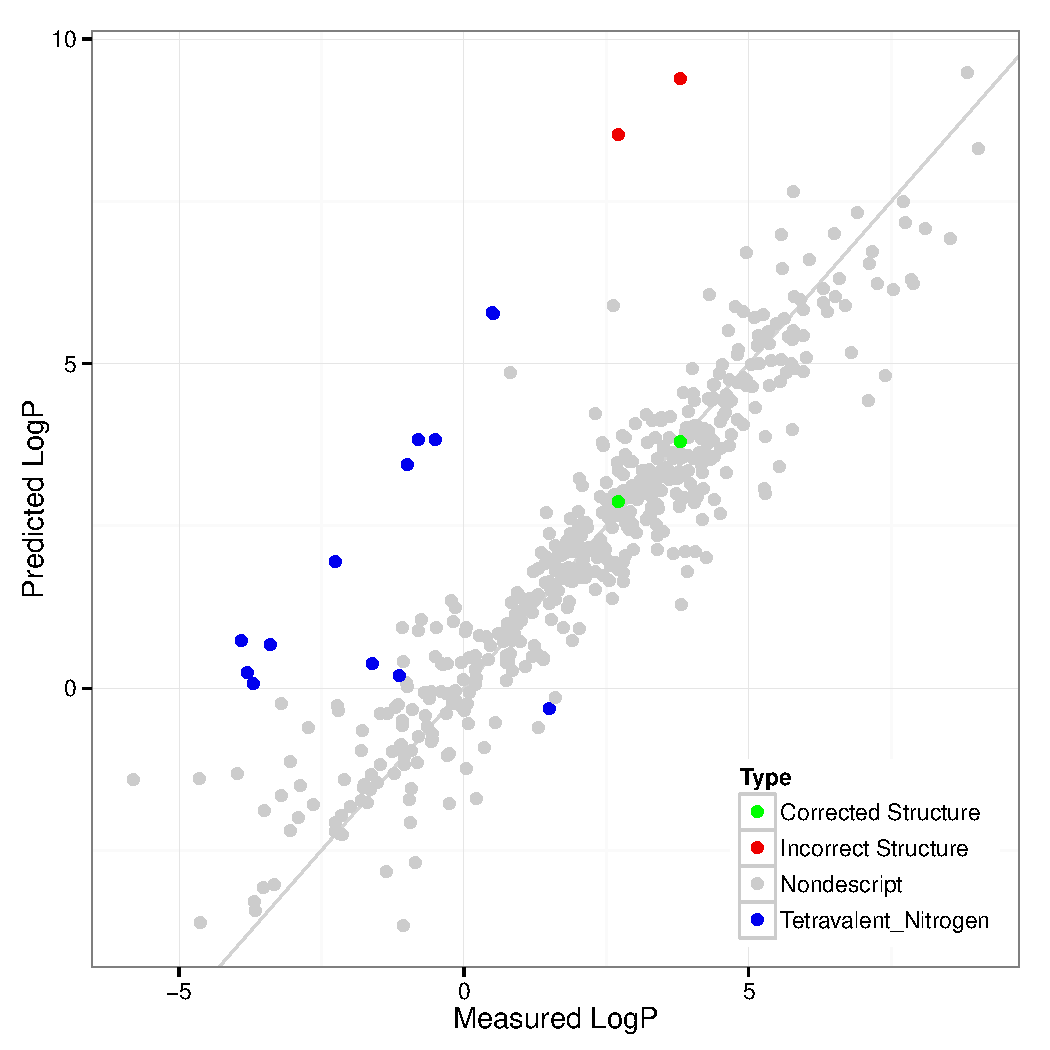
\includegraphics[width=0.6\textwidth]{./figures/error_analysis.pdf}
%\quad
%\subfigure{\includegraphics[width=0.4\textwidth]{./figures/target_density_comparison.pdf} }}}
%\caption{Left: Correlation plot showing the error in predictions on the external test set. the logP of molecules containing tetravalent nitrogens (blue) are all mostly overpredicted. The prediction of two molecules in the dataset with incorrect structure (red) is vastly more accurate when the correct structures are used (green). Predictions of molecules containing more than 3 Flourines account for one outlier but in general behave reasonably. Predictions in the extremities of logP (below -2.5 and above 7.5) are more prone to error. This may be due to a lack of representation of molecules with logP's in this range in the training set as seen from the density plots of the target values for both data sets. Right: Comparison of the distribution of measuered logP values in the training and external test sets. (TBD: This join of figures is done only for layout purposes so that figures don't migrate too far away from the text.)}
%\label{fig12}
%\end{figure}

% y scrambling
%Y-scrambling was performed to help rule out the possibility of chance correlations driving model training (SI figure 1). Y-scrambling works by retraining the model multiple times, but each time randomising or scrambling the target values. If the models trained using the scrambled data perform comparably to the model trained using the non-scrambled data, then the method could be picking up chance correlations. Since the number of training points were many magnitudes larger than the number of variables used, this was only a slight concern. SI figure 1 shows the R Squared and RMSE measures for the scrambled vs non-scrambled data to lie so far apart that the model appears to be representing real correlations within the non-scrambled data.

%\subsection*{Estimating Error in Experimental Measurements} left out because the error's might actually be caused by rounding...
%After standardisation, identical molecules (by canonical SMILES) in training and external datasets were assumed to come from the same original source of experimental data if the logP values matched exactly. For those molecules that were identical but that had different logP measurements in the external and training datasets, an RMSE was calculated using the two different sets of measurements. This allowed a method of estimation for the logP measurement error between the datasets that can be compared to the prediction error given by any particular modelling algorithm (see figure \ref{fig:measurement_error}).
%
%\begin{figure}[ht]
%  \centering
%  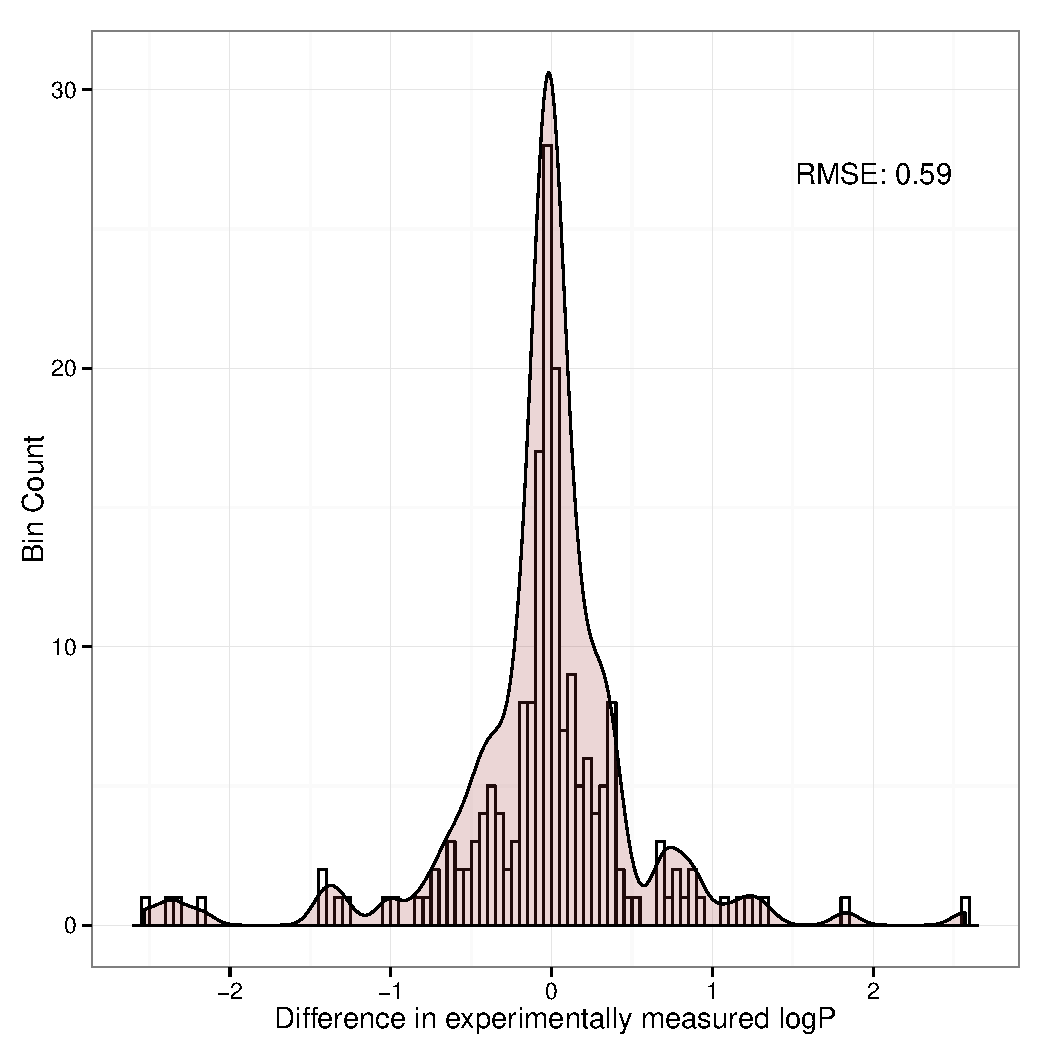
\includegraphics[width=0.60\textwidth]{./figures/measurement_error.pdf}
%  \caption{Histogram of the differences in measurement between identical molecules of the training set and external test set that do not have the same recorded experimentally measured logP value. Y-axis shows the number of molecules in a particular difference range (or bin). This gives an estimate of the error inherent in measurements between the two sets of data.}
%  \label{fig:measurement_error}
%\end{figure}


% The octanol/water partition coefficient (logP)

% require the molecules to be uploaded online.

% two problems with this exist.
% 1. secret molecules can't be uploaded
% 2. it is difficult to integrate this into any sort of work flow

%         % Do not use inserted blank lines (ie \\) until main body of text.
% - no easily integratable method exists that is decent and works off
% free descriptors \\
% - forward selection using various correlation measures (best small set
% of variables can be used for speed improvement) \\
% - correlation methods also help in error estimation \\

% - good predictions (comparison to other models) \\
% - freely available and easily integratable \\
% - comparison to MOE descriptors? (may as well since I've found the
% optimal hyperameters) \\
% - use of variable correlation methods in forward variable selection \\ 
% - GP method doesn't scale up to datasets this large (read this once, 
% need to confirm) \\ IT DOES IT JUST USES A LOT OF MEMORY
% - use of variable correlation methods in error estimation \\
% - error analysis (need to print out worst X predictions and look at
% them) \\

%\cite{koon,oreg,khar,zvai,xjon,schn,pond,smith,marg,hunn,advi,koha,mouse}

\section*{INSTRUCTIONS}
% just before abstract
%%%%%%%%%%%%%%%%%%%%%%%%%%%%%%%%%%%%%%%%%%%%%%
%%                                          %%
%% The Abstract begins here                 %%
%%                                          %%  
%% Please refer to the Instructions for     %%
%% authors on http://www.biomedcentral.com  %%
%% and include the section headings         %%
%% accordingly for your article type.       %%   
%%                                          %%
%%%%%%%%%%%%%%%%%%%%%%%%%%%%%%%%%%%%%%%%%%%%%%

% just before introduction
%%%%%%%%%%%%%%%%%%%%%%%%%%%%%%%%%%%%%%%%%%%%%%
%%                                          %%
%% The Main Body begins here                %%
%%                                          %%
%% Please refer to the instructions for     %%
%% authors on:                              %%
%% http://www.biomedcentral.com/info/authors%%
%% and include the section headings         %%
%% accordingly for your article type.       %% 
%%                                          %%
%% See the Results and Discussion section   %%
%% for details on how to create sub-sections%%
%%                                          %%
%% use \cite{...} to cite references        %%
%%  \cite{koon} and                         %%
%%  \cite{oreg,khar,zvai,xjon,schn,pond}    %%
%%  \nocite{smith,marg,hunn,advi,koha,mouse}%%
%%                                          %%
%%%%%%%%%%%%%%%%%%%%%%%%%%%%%%%%%%%%%%%%%%%%%%


%%%%%%%%%%%%%%%%
%% Background %%
%%

% Table generated by Excel2LaTeX from sheet 'results.csv'
%\begin{table}[htbp]
%  \centering
%  \caption{RMSE of various learning algorithms}
%    \begin{tabular}{rrrrr}
%    \toprule
%    Model & Train & CV    & Test  & External \\
%    \midrule
%    MLR   & 0.557 & 0.583 & 0.587 & 1.236 \\
%    KNN   & 0.546 & 0.718 & 0.669 & 1.364 \\
%    PLS   & 0.635 & 0.592 & 0.682 & 1.143 \\
%    RF    & 0.210 & 0.541 & 0.514 & 1.143 \\
%    GPR   & 0.407 & 0.517 & 0.488 & 1.213 \\
%    RVR   & 0.323 & 0.495 & 0.471 & 1.221 \\
%    SVR   & 0.186 & 0.392 & 0.375 & 1.091 \\
%    \bottomrule
%    \end{tabular}%
%  \label{tab:addlabel}%
%\end{table}%

\begin{verbatim}
 > different[which(abs(different$difference) < 0.1),]
                     Name2     Name1 logP_medlin logP_pkkb difference
1                 Abacavir   B063224        1.22     1.200      0.020
2               Acebutolol   B017779        1.71     1.770     -0.060
3            Acetaminophen   B003202        0.51     0.460      0.050
7           Acetophenazine   B004305        3.32     3.418     -0.098
9                  Adenine   B062114       -0.09    -0.050     -0.040
32                Atenolol B008484_0        0.17     0.230     -0.060
34               Azatadine   B034678        3.59     3.600     -0.010
35            Azelaic Acid   B066955        1.57     1.646     -0.076
53              Budesonide B018313_0        3.20     3.145      0.055
56                Busulfan   B046079       -0.52    -0.500     -0.020
57            Butabarbital   B016136        1.65     1.631      0.019
97              Clobetasol   B014745        2.47     2.480     -0.010
118           Debrisoquine   B057874        0.75     0.800     -0.050
121          Dexamethasone B014746_0        1.74     1.830     -0.090
135               Dopamine   B060329        0.51     0.548     -0.038
136              Dosulepin   B032479        4.49     4.520     -0.030
144                Estriol B014311_0        2.54     2.450      0.090
146                Ethanol   B027357       -0.31    -0.300     -0.010
148               Ethotoin   B026595        1.05     1.083     -0.033
154             Famotidine   B058040       -0.80    -0.726     -0.074
155             Famotidine   B059483       -0.64    -0.726      0.086
166           Flumethasone B014711_0        1.94     1.900      0.040
167          Flunitrazepam   B035318        2.06     2.100     -0.040
168 Fluocinolone Acetonide   B014845        2.47     2.500     -0.030
175           Fluspirilene   B056757        5.86     5.900     -0.040
183           Griseofulvin B038755_0        2.18     2.150      0.030
195         Hydrocortisone B012197_0        1.61     1.692     -0.082
199              Ibuprofen B008055_0        3.50     3.481      0.019
207              Isoniazid   B060557       -0.70    -0.640     -0.060
218             L-Cysteine   B059256       -2.49    -2.500      0.010
224              L-Proline   B066456       -2.50    -2.540      0.040
225            L-Threonine B011111_0       -2.94    -2.980      0.040
237              Lorazepam   B069395        2.39     2.450     -0.060
244              Malathion   B028031        2.38     2.360      0.020
248        Mechlorethamine   B034015        0.90     0.910     -0.010
252              Meloxicam   B035278        3.01     3.020     -0.010
259            Mepivacaine B034877_0        1.95     1.900      0.050
264            Metaraminol   B010570       -0.29    -0.270     -0.020
273         Methoxyflurane   B038648        2.21     2.200      0.010
278             Meticillin   B042216        1.22     1.200      0.020
279           Metildigoxin   B038823        1.73     1.800     -0.070
281         Metoclopramide   B025919        2.62     2.640     -0.020
309             Nitrazepam   B064800        2.13     2.190     -0.060
311         Nitrofurantoin   B064624       -0.47    -0.500      0.030
316             Nordazepam   B054568        2.93     2.900      0.030
324             Oxprenolol   B008549        2.10     2.180     -0.080
331             Penbutolol B005080_0        4.06     4.150     -0.090
338             Phenacetin   B029617        1.65     1.580      0.070
345    Phenylpropanolamine B010571_0        0.67     0.700     -0.030
358             Prednisone   B012175        1.47     1.500     -0.030
362           Procainamide   B025940        0.98     0.880      0.100
373           Propoxyphene B015498_0        4.18     4.200     -0.020
374           Pyrazinamide   B058811       -0.60    -0.550     -0.050
383            Ropivacaine   B024049        2.90     2.890      0.010
388         Salicylic_acid B068016_0        2.26     2.326     -0.066
396          Sulfacetamide   B003071       -0.96    -1.000      0.040
398       Sulfadimethoxine   B043398        1.63     1.600      0.030
400          Sulfaethidole   B031087        1.01     1.000      0.010
402         Sulfamethazine   B050319        0.89     0.900     -0.010
405          Sulfanilamide   B061524       -0.62    -0.600     -0.020
408          Sulfisomidine   B050376       -0.33    -0.300     -0.030
410              Sulpiride   B026849        0.64     0.620      0.020
428                Timolol   B005088        1.83     1.910     -0.080
429             Tinidazole   B030119       -0.36    -0.350     -0.010
434               Tolmetin   B048389        2.79     2.800     -0.010
437          Triamcinolone   B014173        1.16     1.200     -0.040
439        Trifluoperazine   B035618        5.03     5.000      0.030
443      Trimethobenzamide   B040573        2.29     2.300     -0.010
446           Triprolidine   B048348        3.92     3.900      0.020
447            Tropicamide   B026548        1.28     1.200      0.080
451               Xipamide   B048816        2.19     2.200     -0.010
\end{verbatim}


